\documentclass{article}
\usepackage{harpoon}  % used for vector arrow notation
\usepackage{multicol}
\usepackage{graphicx}
\usepackage[rightcaption]{sidecap}


\title{\vspace{-4cm}
Quantum Computing Cheat Sheet
}

\author{ \vspace{-2cm}
Tony Askar
}

\date{} % Removes the default date from the title

\begin{document}
\graphicspath{ {./images/} }

\maketitle
\hrule
\vspace{5pt}

\textbf{bra-ket notation:} Quantum states are represented by column vectors, called kets
\begin{center}
$ |{\psi} \rangle = \left( 
				\begin{array}{c}
					 {\alpha}\\
					 {\beta}
				\end{array} 
			\right)$
\end{center}

\noindent To get a bra from a given ket, we take the conjugate transpose of the ket. (this is known as dagger)
\begin{center}
$\langle{\psi}| = |{\psi} \rangle^\dagger = 
			 \left(
				 \begin{array}{c} 
				 	{\alpha}\\
					{\beta}
				\end{array} 
			\right)^\dagger = \left( \begin{array}{c c} {\alpha}^* &  {\beta}^* \end{array} \right)$\\
\end{center}

\hrule 
\vspace{5pt}

\textbf{Inner Product:} Multiplying a bra and a ket is an inner product that yields the projection, or amplitude, of the states onto each other. The inner product yields a scalar output.
\begin{center}
$\langle{\psi} | {\psi}\rangle = \left( 
						\begin{array}{c}
						   {\alpha} \\
						   {\beta}
						\end{array}
					   \right)^\dagger 
					   \left( 
					        \begin{array}{c}
					            {\alpha} \\
						   {\beta}
						\end{array}
				           \right) = \left(\begin{array}{l r} {\alpha}^*  & {\beta}^* \end{array} \right) 
				                        \left(\begin{array}{c c}{\alpha} \\  {\beta}     \end{array}\right)$


$\langle{\phi} | {\psi}\rangle = \left( 
						\begin{array}{c c} 
							{\gamma} \\
							{\delta}
						\end{array}
					    \right)^\dagger 
					    \left( 
					    	\begin{array}{c}
							{\alpha} \\
							{\beta}
						\end{array}
					    \right) = \left( \begin{array}{lr} {\gamma}^* & {\delta}^* \end{array}\right) 
					    \left( \begin{array}{c c}{\alpha} \\ {\beta}\end{array}\right)$

\end{center}

\begin{itemize}
	\item A state whose inner product with itself equals 1 is normalized.
	\item States with inner product equaling 0 are orthogonal.
\end{itemize}

\hrule 
\vspace{5pt}

\textbf{Outer Product:} Multiplying a ket and a bra is an outer product, which is a square matrix.

\vspace{5pt}
\hrule 
\vspace{5pt}


\textbf{Euler's formula:}
\begin{center}
$ e^{i\theta} = \cos(\theta) + i\sin(\theta) $
\qquad
$ e^{-i\theta} = \cos(\theta) - i\sin(\theta) $
\end{center}

\vspace{5pt}
\hrule
\vspace{5pt}


\textbf{Quantum gates \& Matrices:}

\begin{itemize}
	\item Quantum gates are unitary matrices, which satisfy: $UU^\dagger = U^\dagger U = I$
	\item Unitary matrices are always reversible with: $U^{-1} = U^\dagger$
\end{itemize}

The dagger operation on a matrix, is the conjugate transpose:  $A^\dagger= (\overline{A})^T$

Transpose of a Matrix A:
\begin{center}
$
  A_{3\times3} =
  \left[ {\begin{array}{ccc}
    a & b & c \\
    d & e & f \\
    g & h & i \\
  \end{array} } \right]
$
\qquad
$
  A^T =
  \left[ {\begin{array}{ccc}
    a & d & g \\
    b & e & h \\
    c & f & i \\
  \end{array} } \right]
$
\end{center}

An example of dagger operation:

\begin{center}
$
  A_{2\times2} =
  \left[ {\begin{array}{cc}
    1 + i & 3i \\
    0 & 3 - i \\
  \end{array} } \right]
$
\qquad
$
  A^\dagger =
  \left[ {\begin{array}{cc}
    1 -i & 0 \\
    -3i & 3 + i \\
  \end{array} } \right]
$
\end{center}

\begin{itemize}
	\item \textbf{Trace of a matrix} is the sum of all diagonal elements.
\end{itemize}

\newpage

\textbf{Common gates:}

Identity and Hadamard gates:
\begin{center}
$
  I =
  \left[ {\begin{array}{cc}
    1 & 0 \\
    0 & 1 \\
  \end{array} } \right]
$
\quad
$
  H = \frac{1}{\sqrt{2}} \left[ {\begin{array}{cc}
    1 & 1 \\
    1 & -1 \\
  \end{array} } \right]
$
\end{center}

Pauli gates:
\begin{center}
$
  X = \left[ {\begin{array}{cc}
    0 & 1 \\
    1 & 0 \\
  \end{array} } \right]
$
\quad
$
 Y = \left[ {\begin{array}{cc}
    0 & -i \\
    i & 0 \\
  \end{array} } \right]
$
\quad
$
  Z = \left[ {\begin{array}{cc}
    1 & 0 \\
    0 & -1 \\
  \end{array} } \right]
$
\end{center}

Phase gate:
\begin{multicols}{2}
$ P_{\phi} = \left[ {\begin{array}{cc}
    1 & 0 \\
    0 & e^{i\phi} \\
  \end{array} } \right]$

\columnbreak

$ |0\rangle \rightarrow |0\rangle$

$ |1\rangle \rightarrow e^{i\phi} |1\rangle$
\end{multicols}


\vspace{5pt}
\hrule
\vspace{5pt}


\textbf{Gate identities:} \\

Pauli identities:
\begin{multicols}{2}
	\begin{enumerate}
		\item $ XY = iZ $
		\item $ YZ = iX $
		\item $ ZX = iY $
	\columnbreak
		\item $ XZ = -iY $
		\item $ ZY = -iZ $
		\item $ YX = -iZ $
	\end{enumerate}
\end{multicols}

\begin{multicols}{2}
Hadamard identities:
	\begin{enumerate}
		\item $ HZH = X $
		\item $ HYN = -Y $
		\item $ HXN = Z $
	\end{enumerate}
\columnbreak

S identities:
	\begin{enumerate}
		\item $ SXS^\dagger = Y $
		\item $ SYS^\dagger  = -X $
		\item $ SZS^\dagger  = Z $
	\end{enumerate}
\end{multicols}

\vspace{5pt}
\hrule
\vspace{5pt}
\textbf{Qubit basis states:}

\begin{center}
$ |0\rangle =  \left(
				\begin{array}{c}
					 1 \\
					 0
				\end{array}
			\right)
$
\quad
$ |1\rangle =  \left(
				\begin{array}{c}
					 0 \\
					 1
				\end{array}
			\right)
$
\end{center}

\begin{center}
$H|0\rangle = |+ \rangle =  \frac{1}{\sqrt{2}} |0\rangle + \frac{1}{\sqrt{2}}|1\rangle$

$H|1\rangle = |- \rangle = \frac{1}{\sqrt{2}} |0\rangle - \frac{1}{\sqrt{2}}|1\rangle$
\end{center}

\vspace{5pt}
\hrule
\vspace{5pt}

\newpage


\textbf{Density Matrix:} A general way of expressing a quantum state.
When state vectors and wave functions can only describe pure states, a density matrix can describe mixed states as well.

A density matrix is defined as:

\begin{center}
$ \displaystyle \rho = \sum_{j} P_{j}  |{\psi}_{j} \rangle \langle{\psi}_{j} | $
\end{center}
where $P_{j}$ is the probability of obtaining the state $|\psi_{j} \rangle$. \\

Every density matrix can also be written as a linear combination of Pauli gates, as follows:

\begin{center}
$\rho = \frac{1}{2} I + c_{1} X + c_{2}Y + c_{3}Z$ \\
\end{center}

where  $c_{1}, c_{2}, c_{3}$ give us the Bloch vector in cartesian coordinates:
\begin{center}
$\overrightharp{r} = (x, y, z) = (2c_{1}, 2c_{2}, 2c_{3})$
\end{center}


\vspace{5pt}
\hrule 
\vspace{5pt}


\textbf{State Purity:} a scalar quantity to measure how pure a state is:

\begin{center}
$ purity = \gamma = tr(\rho^2) $
\end{center}

such that $\gamma$ can be between $\frac{1}{d}$ and 1, where d is the dimension of the Hilbert space.

\begin{center}
$\gamma = 1 \rightarrow $ pure state \\
$\gamma \ne 1 \rightarrow $ mixed state \\
$\gamma = \frac{1}{d} \rightarrow $  completely mixed state. % --> maximally entangled
\end{center}

\textbf{Note:} Pure states lie on the surface of a Bloch sphere, whereas mixed states lie within it. 
so if the length of a Bloch vector $(\sqrt{x^2 + y^2 + z^2} )$ equals 1, then the state is pure. 

 
\vspace{5pt}
\hrule 
\vspace{5pt}


\textbf{Fidelity:} a scalar value to measure the closeness of two quantum states, for example the initial state compared with the final state after going through quantum gates, defined as:

\begin{center}

$ F(|\psi_{i}\rangle, |\psi_{f}\rangle) = | \langle \psi_{i} | \psi_{f}\rangle | ^2 $ 

\end{center}

Fidelity holds the following properties:

\begin{itemize}
	\item \textbf{Symmetery:}  $ F(|\psi_{i}\rangle, |\psi_{f}\rangle) = F( |\psi_{f}\rangle, |\psi_{i}\rangle ) $
	\item \textbf{Bounded values:}  $ 0 \le F(|\psi_{i}\rangle, |\psi_{f}\rangle) \le 1$ and $ F(|\psi\rangle,|\psi\rangle) = 1 $
\end{itemize}

\vspace{5pt}
\hrule 
\vspace{5pt}


\newpage

\textbf{Bell States:}
Bell states are a set of two qubits that represent the simplest (and maximal) examples of quantum entanglement.
\begin{center}
$|\Phi^+\rangle = \frac{|00\rangle + |11\rangle}{\sqrt{2}}$
\quad
$|\Phi^-\rangle = \frac{|00\rangle - |11\rangle}{\sqrt{2}}$

\quad

$|\Psi^+\rangle = \frac{|01\rangle + |10\rangle}{\sqrt{2}}$
\quad
$|\Psi^-\rangle = \frac{|01\rangle - |10\rangle}{\sqrt{2}}$

\end{center}

Creating a Bell state on a quantum computer can be done using the following circuits:

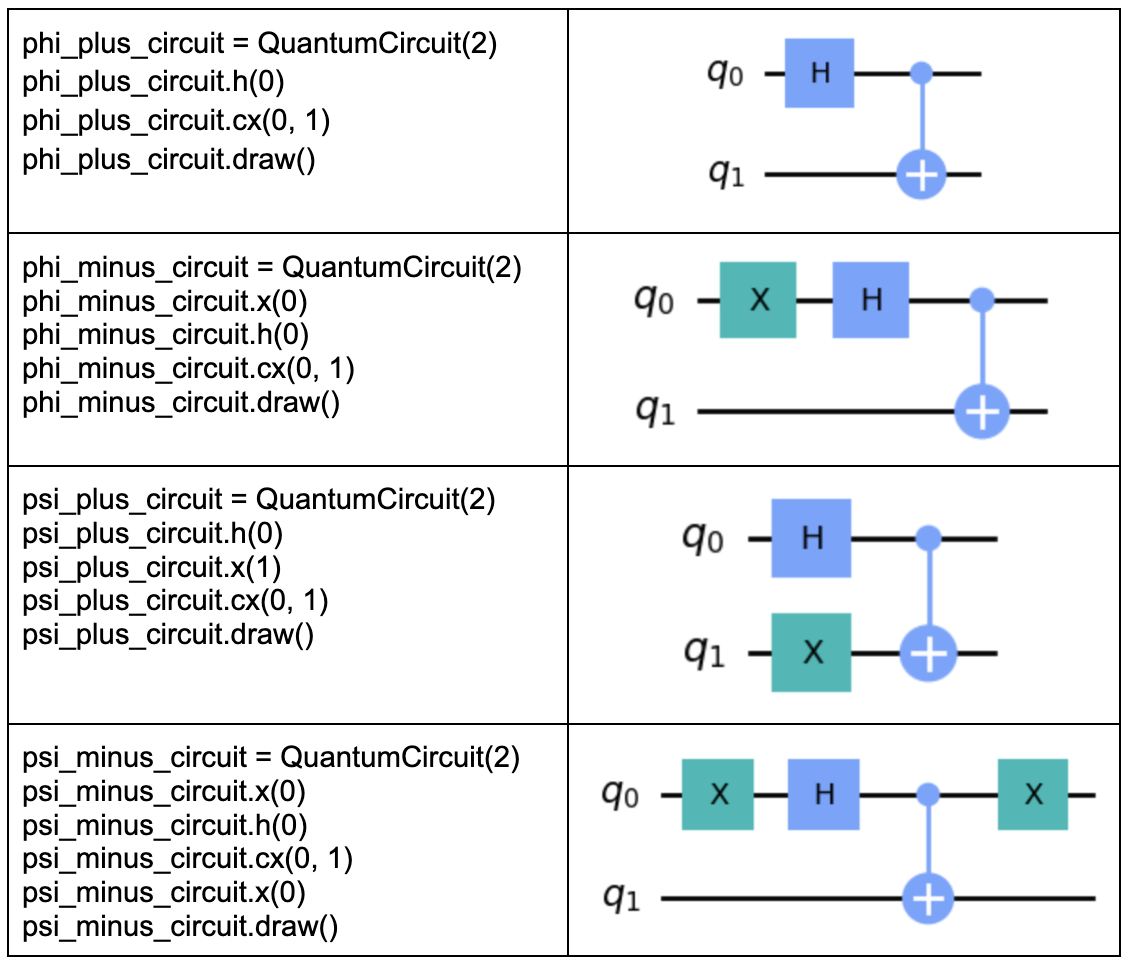
\includegraphics[width=1\textwidth]{bell_states}



\vspace{5pt}

\hrule
\vspace{5pt}



\end{document}